\documentclass[tikz]{standalone}
\usepackage{pgffor}

\begin{document}
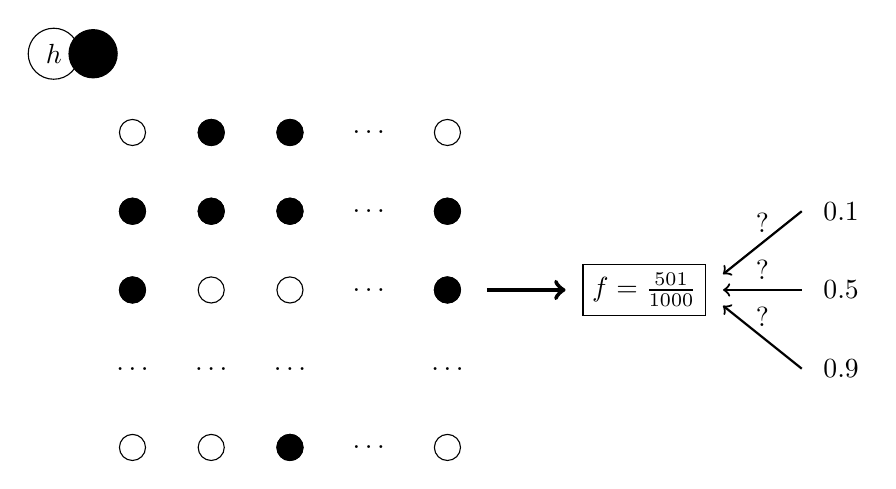
\begin{tikzpicture}

    \node[circle, draw = black] (w) at (0,0) {$h $};
    \node[circle, draw = black,fill=black] (b) at (0.5,0) {$ b$};

    \foreach \x/\n in {1,2,3,5}
    \foreach \y/\m in {1,2,3,5}{
    \node[circle, draw = black] at (\x,-\y) {};
}

    \foreach \x/\y in {1/2,1/3,2/1,2/2,3/1,3/2,3/5,5/2,5/3}{
    \node[circle, draw = black, fill = black] at (\x,-\y) {};
}


    \foreach \x/\n in {1,2,3,5}{
    \node at (\x,-4) {$\dots$};
}

    \foreach \y/\n in {1,2,3,5}{
    \node at (4,-\y) {$\dots$};
}

\draw[ultra thick, ->] (5.5,-3) -- (6.5,-3);
\node[draw] at (7.5,-3) {$f = \frac{501}{1000}$};
\foreach \y/\j/\n in {2/2.8/0.1,3/3/0.5,4/3.2/0.9}{
    \draw[thick, ->] (9.5,-\y) --node[above]{$?$} (8.5,-\j);
    \node at (10,-\y) {\n};
}


    
\end{tikzpicture}
\end{document}